
\item A cubical region of side \( a \) has its centre at the origin. It encloses three fixed point charges, \( -q \) at \( (0, -a/4, 0) \), \( +3q \) at \( (0,0,0) \) and \( -q \) at \( (0,+a/4,0) \). Choose the correct option(s).
    \begin{center}
        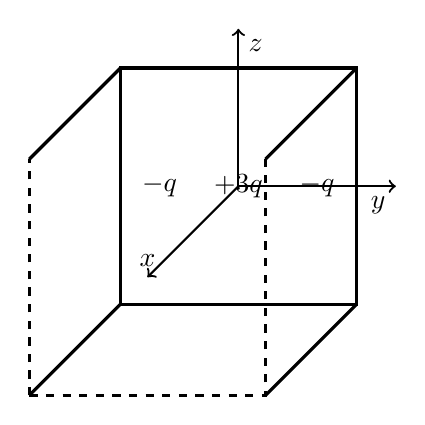
\begin{tikzpicture}
            % Drawing the cube with charges, as a simple representation
            \draw[very thick] (-1.5,-1.5,0) -- (-1.5,1.5,0) -- (1.5,1.5,0) -- (1.5,-1.5,0) -- cycle; % base
            \draw[very thick] (-1.5,-1.5,0) -- (-1.5,-1.5,3);
            \draw[very thick] (-1.5,1.5,0) -- (-1.5,1.5,3);
            \draw[very thick] (1.5,1.5,0) -- (1.5,1.5,3);
            \draw[very thick] (1.5,-1.5,0) -- (1.5,-1.5,3);

            \draw[very thick, dashed] (-1.5,-1.5,3) -- (1.5,-1.5,3) -- (1.5,1.5,3); % top
            \draw[very thick, dashed] (-1.5,-1.5,3) -- (-1.5,1.5,3);

            % Charges
            \node at (-1, 0, 0) { \( -q \) };
            \node at (0, 0, 0) { \( +3q \) };
            \node at (1, 0, 0) { \( -q \) };

            % Axes
            \draw[thick,->] (0,0,0) -- (2,0,0) node[anchor=north east] {\( y \)};
            \draw[thick,->] (0,0,0) -- (0,2,0) node[anchor=north west] {\( z \)};
            \draw[thick,->] (0,0,0) -- (0,0,3) node[anchor=south] {\( x \)};
        \end{tikzpicture}
    \end{center}
    \begin{tasks}(2)
        \task The net electric flux crossing the plane \( x = +a/2 \) is equal to the net electric flux crossing the plane \( x = -a/2 \).
        \task The net electric flux crossing the plane \( y = +a/2 \) is more than the net electric flux crossing the plane \( y = -a/2 \).
        \task The net electric flux crossing the entire region is \( \frac{q}{\varepsilon_0} \).
        \task The net electric flux crossing the plane \( z = +a/2 \) is equal to the net electric flux crossing the plane \( x = +a/2 \).
    \end{tasks}
